Since this work is inspired by \cite{parkendd}, a RegressionTree model was chosen as machine learning method. To keep the complexity of the application in check, the model was kept simple: the data consisted only of timestamped availability data.\todo{explain a little bit more about regression trees}

\subsection{Data Sources}\label{data sources}
The main data source is the actual parking data which is available online. In addition there are other possible features that may influence parking space availability. Since taking all features into account is not possible, this project will solely focus on the parking data in relation to time. 

\paragraph{Parking Usage Live Data}
The homepage of the ASP Paderborn\footnote{City-Managed service for waste management, city cleaning, and parking.} lists the city managed parking areas and the number of currently free parking spots. 
The data is available on \url{https://www.paderborn.de/microsite/asp/parken_in_der_city/freie_Parkplaetze_neu.php}. A more minimal website is available at \url{https://www4.paderborn.de/ParkInfoASP/default.aspx}. 

The website displays 4 attributes: name, type, capacity, and available spots\footnote{respectively: Parkstätte, --, Anzahl, Frei}. After crawling, the parking information will be annotated with the crawling time. The latter will be split into multiple attributes which will be used in the prediction: hour of day \(\hod\), minute of hour \(\moh\), day of week \(\dow\), day of month \(\dom\), week of month \(\wom\), week of year \(\woy\), and \(\yyy\)\footnote{the year is included as a way to keep samples unique in case the project runs more than 1 year.}.

The number of available parking spaces is be called \(y\). With the features defined before, the training data will be a set of tuples of the form  
\[
(\hod, \moh, \dow, \dom, \wom, \woy, \yyy, y)\text{.}
\]

\paragraph{Other data-sources}
It was also considered to enrich the data set by adding event and holiday data as both could influence the parking situation near the city center. In some cases, these events take place on one of the parking areas or directly besides them. However, as most of the big events do not happen while the course ``Practical Project in Machine Learning'' takes place, they will not considered further.

\begin{figure}
  \centering
  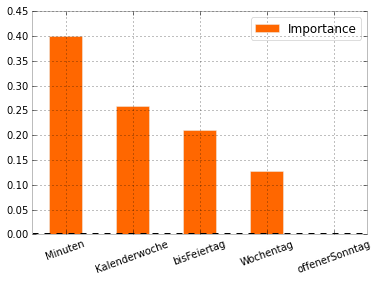
\includegraphics[scale=0.5]{parkendd-Feature-Importance.png}
  \caption{Importance of Features (ParkenDD)}
  \label{fig:parkendd_features}
\end{figure}

Public holidays like Christmas and Easter may also influence the availability of parking space. \cite{parkendd} modeled this in the feature ``bisFeiertag'', i.e. working days until public holiday. In figure \ref{fig:parkendd_features}, the relevance of the different features used by \cite{parkendd} is displayed\footnote{respectively: minutes, week of year, working days until public holiday, day of week, Sunday openings}. 

The feature was relatively important in the evaluation done by \cite{parkendd}. Nonetheless, it will not be included as the next public holiday is Christi Himmelfahrt on 25th May 2017. Therefore there would be no possibility of verifying the importance of this feature in time.

Weather data was also considered as an additional source of information because, e.g., more people may decide to take the car when it's raining. Although such data is available online in machine-readable formats, it will not be considered to keep the model simple.

\subsection{Hypothesis \& Training Method}\label{sec:training_model}

It is assumed, that the available parking space is dependent on time, i.e. there exists a function \(f\) such that 
\[
f(\hod, \moh, \dow, \dom, \wom, \woy, \yyy) = y\text{.}
\]

As mentioned in previous sections, the idea to predict available parking space was inspired by other projects. \cite{parkendd} was using a RegressionTree model with great success, so I picked this model.

To keep the scope of this project small, multiple data sources will be ignored. For this project, it is assumed that the number of available parking spots solely depends on time. As described in \ref{data sources}, this obviously is a very simplified model. However, as shown by \cite{parkendd}, such a simple model may be enough. 

%The greatest challenge in this project is to collect enough training data to make meaningful predictions. All data needs to be extracted from ASP's website. Changes to the website and non-availability of the service may prove problematic. In the beginning of February, the ASP parking guiding system was dysfunctional and did not show useful data for one week. 


\subsection{Comparison between methodologies, if applicable}
The smile library provides different \href{http://haifengl.github.io/smile/index.html}{learning models for Linear Regression}. After a few experiments, the predictions of three models -- GradientTreeBoost, RandomForests, and RegressionTrees -- were ``not completely off''. Since I do not have 
any previous experience in Machine Learning, the prediction module was implemented to train evaluate multiple models 
with different parameterizations on the crawled data and pick the one with the minimum mean average error to make a 
prediction.  

Currently, there are 8567 predictions in total\footnote{Checked on 11.03.2017 at 7:30pm.}. In the course of the 
project GradientBoostTrees turned out to be the dominating prediction model with 7755 predictions. Only 99 of the 
predictions made by the system were derived from RandomForests and 713 were derived from using a RegressionTree. In the latest 48 hours of predictions, only GradientBoostTrees were chosen as the best model for prediction. 